% !TeX spellcheck = de_DE
\section{Umsetzung des Anforderungskatalogs}\label{sec:umsetzung}
	\subsection{Datenbank}\label{sec:umsetzung:DB:DBS}
		\subsubsection{Datenbankschema}\label{sec:umsetzung:DB:Schema}
		Das Datenbankschema war zum Teil bereits gegeben. Hinzu kamen die Abschnitte zu Nutzer\_innen und Bestellungen. Um auch bei Änderungen des Preises in Bestellungen den Kaufpreis eines Buches in einer bestimmten Bestellung nicht zu verlieren, existiert die Tabelle OrderItem, die den zum Kauf gültigen Preis sichert.
		
		Nutzer\_innen halten über eine 1:n-Verbindung beliebig viele Orders, die wiederrum beliebig viele OrderItems beinhalten. Zudem ist die Tabelle User über eine Zwischentabelle mit Books assoziiert, in der verschiedene user- und buchspezifische Daten gespeichert sind. In der aktuellen Umsetzung sind das die Anzahl an Aufrufen eines bestimmten Buches über einen bestimmten Account sowie das Datum des letzten Aufrufs.
	
	
\begin{figure}[h]
\centering
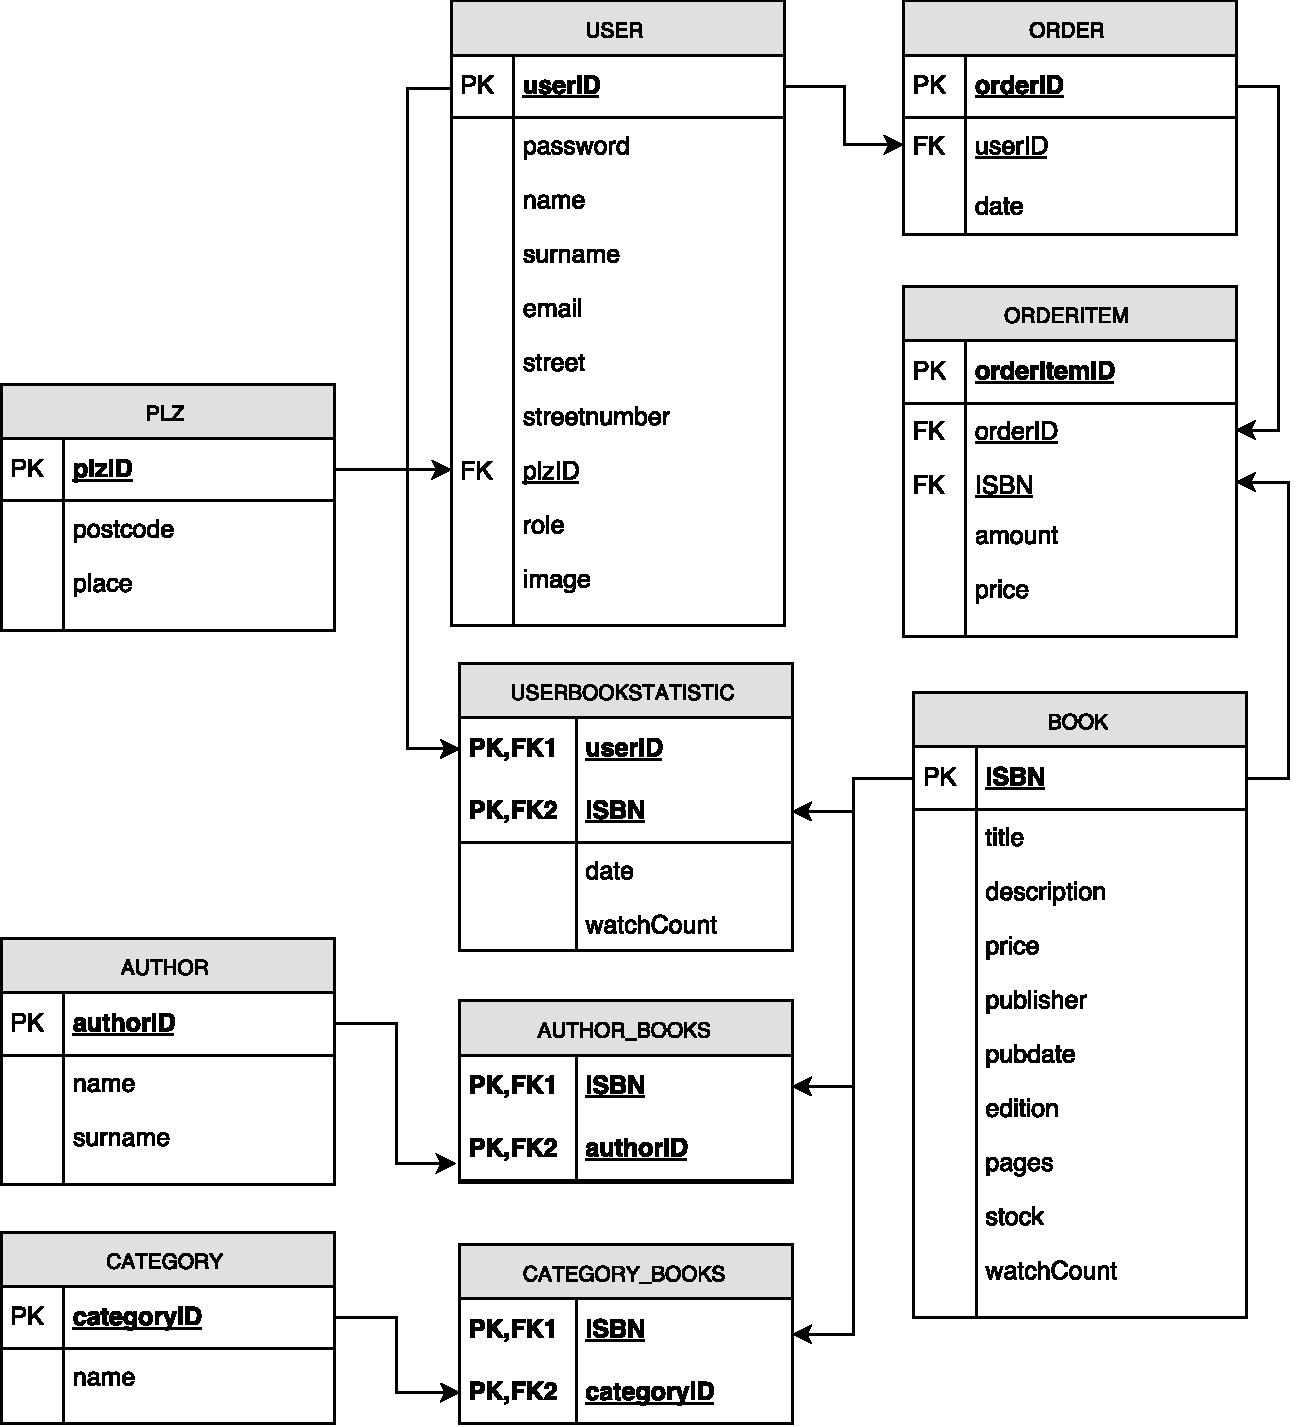
\includegraphics[width=\linewidth]{files/db-schema}
\caption{Das Datenbankschema von \textit{kirjanystaevaet}}
\label{fig:db-schema}
\end{figure}

	
	\subsection{A1: Datenmanagement}\label{sec:umsetzung:DB:DM}
	Grundlage der Datenverwaltung von \textit{kirjanystaevaet} ist die Java-SQL-Datenbank H2. Sie bietet in unseren Augen die für unsere Anforderungen beste Gewichtung von Funktionsumfang und Nutzungsfreundlichkeit. Zum einen ist die Datenbank selbst klein, zum anderen ohne größere Probleme und zusätzliche Fragestellungen (Server etc.) einzurichten. Trotzdem kann bei Bedarf auch eine kompliziertere Konfiguration vorgenommen werden. Die Datenbank von \textit{kirjanystaevaet} läuft auf dem gleichen Server wie die Anwendung selbst. Das Programm greift dabei lokal auf die Daten zu, startet dabei aber den H2 inhärenten Server, sodass theoretisch auch andere Software die Datenbank gleichzeitig nutzen könnten. Im aktuellen Anwendungsfall ist dies aber zu vernachlässigen.
	
	In \textit{kirjanystaevaet} schließlich kommt Hibernate für objektrelationales Mapping zum Einsatz. Ziel ist es, einem Datensatz aus der Datenbank ein Java-Objekt zuzuordnen. Die Entscheidung zu dieser Vorgehensweise fiel vor allem aus persönlichem Interesse sowie aus Erfahrungen mit der Programmierung von rein SQL-basierten Anwendungen und den damit verbundenen Schwierigkeiten, kompliziertere Datenbankanfragen dynamisch zu konstruieren. Zudem sind viele Standards in Verbindung mit Datenbankabfragen (Prepared Statements etc.) von Seiten Hibernates bereits umgesetzt und müssen nicht im eigenen Code geschrieben werden. Zwar kann es bei größeren Abfrageergebnissen mit vielen genesteten Objekten (bei ManyToMany-Verbindungen) bei unvorsichtiger Konfiguration schnell zu großen (unnützen) Datenmengen kommen, bei der abzuschätzenden Größe des Büchershops sollten sich diese Probleme jedoch im Rahmen halten. Wie im folgenden beschrieben, wurde im Programm dennoch eine überlegte Verwendung der FetchTypes eager und lazy angestrebt.
		
		\subsubsection{Architektur der Datenbankfunktionen}\label{sec:umsetzung:DB:Funktionen}
		Da in diesem Projekt Hibernate verwendet wird, wurde für jede Entität eine Klasse erstellt, die alle Daten anhand von Instanzvariablen enthält. Verknüpfungen zu anderen Entitäten werden hergestellt, indem eine Entität eine Collection einer anderen Entität hält. Über Annotationen werden die Eigenschaften der einzelnen Spalten definiert. So lässt sich beispielsweise über \texttt{@Id} angeben, dass es sich bei dieser Variable um den Primärschlüssel handelt. In den meisten Fällen werden die Ids beim Einfügen automatisch generiert. Nur in der Klasse \texttt{book} fungiert die ISBN als Schlüssel. Weiterhin werden über die Annotationen die Beziehungen zu anderen Entitäten definiert. Hierbei können ebenfalls verschiedene Einstellungen vorgenommen werden.
		
		Zum einen werden die \texttt{FetchTypes} festgelegt. \texttt{LAZY} bedeutet hierbei, dass die verknüpften Entitäten bei einer Datenbankabfrage nicht mitgeladen werden. Das wurde hier bei \texttt{books} in \texttt{Category} so gehandhabt. Wenn man z.B. nur die Liste aller vorhanden Kategorien aus der Datenbank abfragen will, werden die einzelnen Bücher häufig gar nicht benötigt. Bei dieser Einstellung werden sie nicht mitgeladen und so der Datentransfer klein gehalten. Um die Bücher einer Kategorie zu bekommen, wird eine gesonderte Abfrage gemacht. Anders sieht es bei \texttt{authors} in \texttt{Book} aus. Diese werden häufig benötigt und da es sich nicht um viele Autor-Datensätze pro Buch handelt, stellt es keinen Nachteil dar, sie sofort aus der Datenbank zu laden. Dafür wird der \texttt{FetchType} auf \texttt{EAGER} gesetzt. Bei allen Verknüpfungen, die mit \texttt{User} und \texttt{Order} zusammenhängen, verhält es sich ebenso.
		
		Außerdem wird der \texttt{CascadeType} bestimmt. So wird geregelt, dass wenn z.B. das letzte Buch einer Kategorie gelöscht werden sollte, die entsprechende \textit{Category} nicht ebenfalls gelöscht wird, da diese einen hohen Wiederverwendungswert haben. Andererseits würde ein \texttt{Author} eines Buches gelöscht werden, wenn er mit keinem Buch sonst mehr verknüpft ist (allgemein zum Löschen von Büchern siehe \ref{umsetzung:DB:Loeschen}).
		
		Die Datenbankzugriffe finden in den \textit{Data Access Objects (DAOs)} statt, die es für jede Entität gibt. Diese sind mit einer \textit{@Trans\-actio\-nal}-Annotation versehen, die die programmatische Umsetzung von Öffnung, Schließung und möglicherweise notwendigen Rollbacks von Transaktionen obsolet macht. Nur in seltenen Fällen enthalten die \textit{DAOs} Logik. Eine Ausnahme ist die \texttt{createOrder}-Methode im \texttt{OrderDao}, da im Zuge einer Bestellung auch der Bestand angepasst werden muss und Konsistenz sichergestellt sein muss (siehe \ref{umsetzung:Suche}). Einzelne Methoden der \textit{DAOs} sind mit \lstinline|@SuppressWarnings("unchecked")| versehen. Da die Datenbankabfragen Werte einer Tabelle und damit eine Menge von gleichen Objekten zurückliefern, kann von einer sicheren Umwandlung in die entsprechenden Listen ausgegangen werden.
		
		Der Aufruf der \textit{DAOs} erfolgt über die \textit{Services}. Diese enthalten die grundsätzliche Logik und das Exception Handling (siehe \textbf{ref}). An dieser Stelle werden Daten verarbeitet, in eine andere Form gebracht und bei Bedarf sortiert und dann eine Schicht weiter nach oben gegeben. Unter anderem deshalb sind die \textit{Services} sehr viel umfangreicher als die \textit{DAOs}. Außerdem fassen sie mehr zusammen, da beispielsweise der \texttt{DataService} alle Funktionen für die Verarbeitung der Entitäten \texttt{Book}, \texttt{Category} und \texttt{Author} enthält, da diese sehr stark zusammenhängen. Weiterhin gibt es einen \texttt{OrderService} für die Verwaltung der Entitäten \texttt{Order} und \texttt{OrderItem}. Die Funktionalität, die den \texttt{User} betreffen, befinden sich im \texttt{UserService}. Im Verlauf des Projekts wurde häufig diskutiert, welche Datentypen der \textit{Service} weiter geben darf und ob es zu Problemen kommen kann, wenn direkt die Entitäten der Objekte weiter gereicht werden. Es wurde entschieden, dass die Objekte weitergegeben werden, allerdings wurden sie mithilfe von \textit{Buildern} als (weitgehend) \texttt{immutable} konstruiert. Dadurch soll vor allem verhindert werden, dass zum einen zur Laufzeit mit verfälschten Objekten gearbeitet wird sowie aufgrund von falschen Annahmen zur Funktionsweise dieser Objekte mögliche Änderungen nur am Objekt vorgenommen, aber letztendlich nicht in der Datenbank gespeichert werden.
		 
		Ein hilfreiches Mittel zum Datenaustausch sind weiterhin die \textit{Enum}, die die Felder der Entitäten, bzw die Spalten der Datenbanktabellen abbilden. Ein gutes Beispiel für die Verwendung der \textit{Enums} ist die \texttt{insertBook}-Methode des \texttt{DataService}. Hier werden dem \texttt{Service} über eine \texttt{Map\textless Searchfields, String\textgreater } alle notwendigen Daten übergeben, wobei das Enum im Key die Zugehörigkeit der Daten im Value angibt. Auch bei der Suche über Metadaten werden die Daten auf diese Weise an den \textit{Service} übergeben.
		
		\subsubsection{Einfügen von Daten}\label{umsetzung:DB:Einfuegen}
		Soll ein Buch eingefügt werden, ist es wichtig, dass die zugehörigen Kategorien und Autoren schon vorher in der Datenbank gespeichert sind. Autoren erfahren hier außerdem eine spezielle Behandlung. Soll ein neuer Autor eingefügt werden, wird überprüft, ob es schon einen Autor mit exakt diesem Namen gibt und wenn ja, nochmals nachgefragt, ob es sich tatsächlich um eine neue Person handelt oder vielleicht eine der schon vorhandenen gemeint ist. Das trägt der Tatsache Rechnung, dass auch die Kombination von Vor- und Nachnamen keineswegs eindeutig sind. 
		
		Das Anlegen neuer Accounts muss verschiedene Sicherheitseinstellungen in Rechnung nehmen. Zum einen ist es elementar, dass angegebene Passwort verschlüsselt in die Datenbank zu legen. Dafür sorgt der auf der bcrypt-Hashfunktion bassierende \texttt{BCrypt\-Password\-Encoder}. Zum anderen werden User über entsprechende Enums in Admin und User unterteilt, um verschiedene Rollen und Berechtigungen zuweisen zu können. Die in Deutschland verfügbaren Postleitzahlen sind bereits in der Datenbank hinterlegt. Eine zusätzliche Anlegung ist über das entsprechende \textit{DAO} prinzipiell möglich, auf Ebene der \textit{Services} jedoch nicht weiter verfolgt. Zusätzlich zu den im Katalog geforderten Funktionen ist zudem experimentell die Speicherung eines Profilbildes als Bytestream ermöglicht.
		
		\subsubsection{Löschen von Daten}\label{umsetzung:DB:Loeschen}
		Das Löschen von Daten ist nur eingeschränkt möglich. Prinzipiell bieten die \textit{DAOs} die entsprechenden Funktionen dafür an. Zumindest bei Büchern werden sie von der entsprechenden Methode im Service jedoch nicht verwendet. Da es ein Bestell-Archiv gibt, das heißt jeder User kann jede Bestellung, die einmal getätigt wurde, einsehen, ist es nicht möglich die Datensätze zu löschen, auch wenn das Buch nicht mehr angeboten wird. In welchen Zustand sich ein Buch befindet wird über die Spalte \texttt{stock} geregelt. Im Prinzip zeigt diese an, wie viele Exemplare von einem Buch vorrätig sind, ist der Wert jedoch negativ, bedeutet das, dass das Buch nicht mehr verkauft wird. Ruft man im Service also die \texttt{deleteBook}-Methode auf, wird nur der \texttt{stock} auf \texttt{-1} gesetzt.
		
		Daraus folgt, dass auch Kategorien und Autoren nicht gelöscht werden können, da dies nur möglich wäre, wenn keine Bücher mehr vorhanden wären, die mit dem jeweiligen Datensatz verknüpft sind.
		
		\subsubsection{Ändern von Daten}\label{umsetzung:DB:Aendern}
		Ursprünglich war vorgesehen, dass nur sehr wenig an Büchern geändert werden kann, da die meisten Angaben von der ISBN abhängig sind. So kann sich beispielsweise der Titel einer Ausgabe nicht ändern. Veränderungen in den Daten, die in diesem Fall in der Datenbank gespeichert werden, erfordern eigentlich auch eine neue ISBN\footnote{siehe hierzu \url{https://de.wikipedia.org/wiki/Internationale\_Standardbuchnummer} unter \textit{Regeln zur ISBN-Vergabe und -Nutzung}}. Solch ein restriktives Vorgehen würde jedoch zu anderen Problemen führen, nämlich dass z.B. Tippfehler, die ein Admin beim Einfügen neuer Bücher macht, nicht ausgebessert werden können. Aus diesem Grund haben wir entschieden, dass bei Büchern alle Daten -~bis auf die ISBN~- geändert werden können und die Verantwortung für korrekte Daten damit dem Admin überlassen bleibt.
	
		\subsubsection{Exception Handling}\label{umsetzung:DB:Exception}
		Im Umgang mit der Datenbank können viele Fehler auftreten. Durch ein umfassendes Exception-Handling wird versucht den Shop vor dem Absturz zu bewahren.
			
		Es wurde viel darüber nachgedacht und diskutiert, wie man die oberen Schichten über Fehler oder unerwartetes Verhalten informieren kann, wenn es geht auch ohne Exceptions. Die Probleme liegen darin, wenn ein einzelnes Objekt in der Datenbank gesucht wird und der Rückgabetyp des entsprechenden Services keine \texttt{List\textless..\textgreater}, sondern vom Typ der entsprechenden Entität ist. Es soll unbedingt vermieden bei einer erfolglosen Suche null zurückzugeben. Ein anderer Fall liegt vor, wenn versucht wird eine Entität zu löschen, die nicht existiert oder eine Entität in die Datenbank zu speichern, die schon existiert. Im Sinne der Nutzerfreundlichkeit ist es sinnvoll, zu informieren, dass ein Objekt nicht gelöscht wurde, da es nicht existiert. Solche Fehler können z.B. durch Tippfehler in der Eingabe entstehen und dann zu unerwartetem Verhalten führen, wie z.B. das Objekt, das eigentlich gelöscht werden sollte, ist immer noch vorhanden.
		
		Eine Idee war es Enums zu verwenden, die den Status eines Vorgangs angeben (z.B. \texttt{delete succssful} o.ä.) und überprüft werden können, um dementsprechend zu handeln. Der gravierende Nachteil dieser Lösung ist, dass sie nur bei \texttt{void}-Methoden anwendbar ist. Aus diesem Grund haben wir uns gegen diese Idee entschieden und sind doch dabei geblieben, bei Fehlern Exceptions zu werfen, um alle Probleme durchgängig einheitlich behandeln zu können.
			
		Dabei haben wir darauf geachtet, so weit es möglich ist, nur eine Exception an die oberen Schichten weiter zu geben, nämlich die \texttt{DatabaseException}. Ihr werden mithilfe des \texttt{ErrorMessageHelpers} sehr spezifische, aber einheitliche Fehlernachrichten mitgegeben, die dann z.B. dem Nutzer, v.a. wenn es sich um den Admin handelt, angezeigt werden können.
		
		Zudem wurde auf diese Weise versucht, \texttt{HibernateExceptions} schon auf der Ebene der \textit{Daos} und \textit{Services} abzufangen und ebenfalls in eine \texttt{DatabaseException} umzuwandeln. Es soll so verhindert werden, dass unchecked Exceptions den Shop zum Absturz bringen.
		
		\subsubsection{Testen der Funktionen der \textit{Services}}
		Für das Testen der Funktionen der \textit{Services} wurde eine \texttt{Main}-Methode, die die \texttt{ServiceTest}-Klasse einbindet, verwendet. Sobald eine Methode in einem \textit{Service} implementiert wurde, wurde im \texttt{ServiceTest} ebenfalls eine Methode programmiert, um die neue Funktionalität zu debuggen und ihre Ergebnisse zu überprüfen. Wurde etwas Grundlegendes an den \textit{Services} verändert, wie beispielsweise die Einführung neuer Items, wurden nochmals alle Testmethoden ausgeführt, um sicherzustellen, dass nicht neue Fehler oder unerwünschte Verhaltensweisen entstanden sind.
		
	\subsection{A2: Frontend}
	Zur Umsetzung des Frontends wurden die anfangs vorgestellten Java Server Pages verwendet, um ein angenehmes Erscheinungsbild zu erreichen, wurde auf das HTML und CSS Framework Bootstrap\footnote{\hyperlink{https://getbootstrap.com}{https://getbootstrap.com}} zurückgegriffen. Zur Verbesserung der Nutzung und Interaktivität des Shops wird an einigen Stellen JavaScript\footnote{Aufgrund der Verwendung von ECMAScript6 ohne die Umwandlung in eine frühere Version wird ein aktueller Browser zur vollständigen Nutzung der Seite benötigt.} und jQuery\footnote{\hyperlink{https://jquery.com}{https://jquery.com}} genutzt.
	
		\subsubsection{Zuordnung von Views und Controllern}	
		Mit einzelnen Ausnahmen besitzt jeder View, das heißt jede im Browser dargestellte Seite, eine eigene \lstinline|.jsp|-Datei und einen eigenen Controller. Einzelne Views können dabei durchaus unterschiedlich auftreten, wie zum Beispiel die Darstellung der Kategorien. Der zuständige Controller erwartet als Pfad-Variable in der URL den gesuchten Kategoriennamen. Kann die Variable einer existierenden Kategorie zugeordnet werden, werden alle Bücher dieser Kategorie angezeigt, andernfalls wird eine Übersichtsseite angezeigt. Beide Darstellungen werden durch den gleichen Controller und \lstinline|.jsp|-Datei erzeugt.
		
		Die für die Anzeige benötigten Daten werden in den Controller-Methoden dem Model hinzugefügt und können anschließend im View abgegriffen werden. Im gesamten Shop werden alle zur Darstellung benötigten Daten auf diese Weise den Views zur Verfügung gestellt. Grundsätzlich werden anonymen Nutzer\_innen und Kund\_innen nur zum Verkauf stehende Bücher angezeigt.
		
		Ausgang für alle späteren HTML-Seiten ist eine grundlegende jsp-Datei, die von allen Views erweitert wird. Die Definition der Views und ihrer Dateien sind in der \lstinline|tiles.xml| festgelegt. Die Struktur ist sehr simpel, auf eine Verschachtelung wurde verzichtet. Das liegt unter anderem an einem zu Beginn fehlendem Konzept, wie die Views sinnvoll gegliedert werden können. Noch ist die Anzahl der entsprechenden Dateien und Beziehungen überschaubar, bei einer Erweiterung des Shops ist ein entsprechendes Konzept unabdingbar.
		
		\subsubsection{Funktionalitäten des Frontends}
		Das Frontend ermöglicht alle grundlegenden Funktionalitäten zur vollständigen Nutzung des Shops. Nutzer*innen können sich registrieren, einloggen, Bücher auswählen und in den Warenkorb legen und schließlich bestellen. Administrator*innen haben im Backend (siehe Kapitel \ref{sec:umsetzung:backend}) alle Möglichkeiten zur umfassenden Verwaltung des Shops und Bestands.
		
		Vom oben beschriebenen Datenfluss weicht die Seite zur Registrierung ab. Da in der Datenbank die Postleitzahlen als Entität abgelegt werden und es zu einer Postleitzahl mehrere Orte geben kann (zum Beispiel bei \lstinline|37627|), muss bei der Registrierung ein eindeutiger Wert an den Server übermittelt werden. Daher wird nach einer Eingabe von fünf Zeichen in das Postleitzahlen-Feld diese per AJAX-Request an den Server übermittelt, der alle zu dieser Postleitzahl gehörenden Orte zurückliefert. War die Abfrage erfolgreich, werden die Orte als Auswahlliste in die Seite eingefügt. Mit Beginn der Abfrage wird ein Hinweis angezeigt, so dass auch bei einem länger dauernden Request der Nutzer über die Hintergrundaktivität informiert ist.
		
		\dots
		
		Cart, detaillierter in \ref{sec:umsetzung:cart}
		
		\dots
		
		\subsubsection{Fehlerbehandlung}
		%TODO mehr mehr mehr!
		Beim Datenbank auftretende Fehler sollen Nutzer*innen möglichst nicht auffallen, so dass der Shopbesuch auch bei einem Fehlverhalten des Systems möglichst nicht unterbrochen und gestört wird. Es wird daher in den meisten Fällen zur Fehlerbehandlung ein server-seitiger Redirect eingesetzt, um Nutzer*innen wieder an eine logische und nachvollziehbare Position zu bringen. Diese Strategie wird nicht beim Fehlschlagen von Aktionen eingesetzt, war zum Beispiel die Registrierung oder der Login nicht erfolgreich, wird ein entsprechende Fehlermeldung ausgegeben.
		
		Tritt ein größerer Fehler auf, der durch keinen Controller gefangen wurde, wird eine Standard-Fehlerseite angezeigt. Diese informiert nur über das Fehlschlagen der letzten Aktion, ohne Details über Interna preiszugeben.

	\subsection{A3: Suchfunktion}\label{umsetzung:Suche}
	Die Suchfunktion wird im \texttt{BookService} angeboten. Hierbei wurde sich auf eine Suche über die Metadaten beschränkt. Im Front-End hat der Nutzer die Möglichkeit nach \textit{Titel}, \textit{Vorname}, \textit{Nachname}, \textit{ISBN}, \textit{Erscheinungsjahr} und \textit{Kategorie} zu suchen. Für Datenbankabfragen allgemein und die Suche im besonderen werden \textit{Criteria} verwendet, da sich auf diese Weise sehr einfach dynamische Anfragen generieren lassen. Bei der Suche werden die Angaben der verschiedenen Felder und-verknüpft und sind durch die Verwendung der \texttt{Restrictions.ilike} case-insensitiv und der Suchterm muss nicht exakt so in der Datenbank stehen, sondern kann von anderen Zeichen umgeben sein.
	Auch wenn es in der Oberfläche nicht genutzt wird, kann die \texttt{getBookByMetadata}-Methode im \texttt{BookService} auch alle weiteren Felder von \texttt{Book} in der Suche berücksichtigen. Bei Bedarf könnte der Webshop sehr einfach um diese Suchmöglichkeiten erweitert werden.
	
	Im Laufe des Projekts wurde auch versucht eine offene Suche zu implementieren. Da dies jedoch mit Schwierigkeiten verbunden war und als zu weitreichend für dieses Projekt betrachtet wurde, wurde dieses Vorhaben fallen gelassen. Dies ist jedoch ebenfalls eine Erweiterungsmöglichkeit für die Anwendung. Eine Möglichkeit für die Umsetzung wäre zum Beispiel die Einbindung von \textit{Lucene}, was auch über \textit{H2}-eigene Methoden möglich ist.

	\subsection{A4: Backend}\label{sec:umsetzung:backend}
	Das Backend ermöglicht die komplette Verwaltung des Shops. Insgesamt stellen die Services mehr Methoden zur Verfügung, als schlussendlich client-seitig im Backend umgesetzt wurden. Wie das Kapitel \ref{sec:umsetzung:analyse} zeigt, könnten durch eine Kombination der derzeit gespeicherten Daten komplexere Analysen ermöglicht werden als die derzeit im Dashboard dargestellten.
	
	Das Backend ist in die Bereiche Dashboard, Bestand, Nutzer\_innen und Bestellungen gegliedert. Im Dashboard findet man eine Übersicht über den Shop, im Bereich Bestellungen eine solche über die aktuell laufenden Bestellungen. Der Bestand und alle Nutzer\_innen können in den jeweiligen Untergliederungen verwaltet werden.
	
		\subsubsection{Dashboard}
		Das Dashboard gibt eine Übersicht über aktuelle Werte und Zustände des Shops. Die Daten werden von einer Bean aus den Services abgefragt, in einer \lstinline|Map| zusammengefasst und an den zuständigen Controller weitergereicht. Bisher werden nur "`statische"' Werte abgefragt und angezeigt, auch wenn die Services bereits mehr Möglichkeiten bieten. Die zwischengeschaltete Bean würde es ermöglichen, die unterschiedlichen Werte in Beziehung zu setzen und damit auch komplexere Statistiken anzuzeigen.
	
		\subsubsection{Bestands- und Nutzer\_innenverwaltung}
		Die Bestandsverwaltung untergliedert sich in die Verwaltung der Kategorien, der Autor\_innen und der Bücher. Diese sind client- und server-seitig in unterschiedlicher Weise umgesetzt. So basiert die Nutzer\_innenverwaltung zu einem großen Teil auf AJAX-Requests, während bei der Bestandsverwaltung das Gegenteil der Fall ist. Im Gegensatz zum Frontend, in dem nur die zum Verkauf stehenden Bücher angezeigt werden, werden im Backend immer alle in der Datenbank vorkommenden Bücher angezeigt.
		
		Ausgang für die unterschiedlichen Implementierungen ist der Ablauf beim Anlegen neuer Autor\_innen gewesen. Existiert ein neu angelegter Autor\_in mit dem gleichen Namen bereits in der Datenbank, muss überprüft werden, ob ein neues Datenbankobjekt mit neuer ID angelegt werden soll oder ob ein Versehen vorliegt. Daher wird der neue Datensatz per POST-Request an den Server gesendet, der ein Anlegen des Datensatzes versucht. Schlägt das fehl -- wahrscheinlich, weil ein solcher Datensatz schon existiert -- werden die Daten an den Client zusammen mit einem Http-Statuscode \lstinline|409| an den Client zurück geschickt. In diesem Fall öffnet sich ein Bestätigungs-Dialog, mit dem das Anlegen bestätigt oder abgebrochen werden kann. Ist ein\_e Autor\_in mit gleichem Namen noch nicht bekannt, wird die Aktion ohne Fehlermeldung durchgeführt. Gibt es server-seitig einen anderen Fehler, wird das client-seitig über ein Popup bekannt gemacht und die Aktion abgebrochen.
		
		Ausgehend davon wurden weitere Teile des Backends über die Verwendung von AJAX-Requests umgesetzt, auch mit dem Hintergrund, eine solche Implementierung auf beiden Seiten kennen zu lernen. Aus Nutzer\_innensicht ist hierbei der Vorteil, dass ohne ein Neuladen der Seite Datensätze geändert oder erstellt werden können und zum Beispiel bei komplexeren Anwendungen das Gefühl einer Desktop-Anwendung entstehen kann. Durch die Verwendung von JavaScript können an den richtigen Stellen Hinweise oder Ergänzungen angezeigt werden, wie zum Beispiel die Auswahl des korrekten Ortes bei der PLZ. Da die Daten für die Auswahllisten jedoch server-seitig beim Rendern der Seiten eingebunden werden, fehlen neu erstellte Datensätze in den anderen Auswahllisten. Einzig beim Löschen von Datensätzen wird immer ein server-seitiger Redirect eingeleitet, sodass die Seite neu gerendert wird und die gelöschten Datensätze nicht mehr vorhanden sind. Die fehlende Aktualisierung könnte durch kombinierte Anfragen umgesetzt werden, sodass bei jeder Datensatzänderung oder -erstellung eine akutalisierte Liste vom Server geholt wird und die entsprechenden Felder ergänzt werden. Eine solche Funktionalität erfordert aber eine komplexere client-seitige Implementierung, auf welcher im Projekt kein Fokus lag.
		
		Der im Projekt vorliegende Bestand sowie die umgesetzten Use Cases sind derzeit sehr beschränkt, sodass das gesamte Projekt noch überschaubar ist. Bei zunehmender Größe und Komplexität empfiehlt sich allerdings ein eigenständiges Konzept für den kompletten client-seitigen Bereich, insbesondere auch für die Verwaltung der Daten im Backend. Hilfreich kann hier zudem die Nutzung eines weiteren Frameworks sein, welches die Anbindung an den Server sowie den Datenfluss übernimmt.
		
		\subsubsection{Bestellungen}
		Die Übersicht über die Bestellungen zeigt derzeit eine einfache Liste aller laufenden Bestellungen, eine Unterscheidung zwischen laufenden und abgeschlossenen Bestellungen gibt es aufgrund der Datenschemas nicht. Ebenfalls ist eine Administration der Bestellungen nicht möglich. Mit zunehmender Bestellanzahl wird eine solche Liste nicht mehr ausreichen, ebenso wenn eine Unterscheidung im Bestellstatus erfolgt. Für den geforderten Use Case und Umfang des Projekts erscheint die derzeitige Umsetzung jedoch als ausreichend. Ähnlich wie bei der Bestellverwaltung würde sich auch hier die Nutzung eines Frontend-Frameworks anbieten.
		
		\subsubsection{Fehlerbehandlung}
		Im Gegensatz zum Frontend werden im Backend die meisten Fehler an die Oberfläche durchgereicht und zur Anzeige gebracht. Dies erfolgt in vielen Fällen durch die Ergänzung des Models um die Fehlermeldung oder das Hinzufügen der Fehlermeldung als URL-Parameter. Beim Rendern der Views werden diese Parameter oder Attribute angefragt und zur Anzeige gebracht.
	
	\subsection{A5: Warenkorb}\label{sec:umsetzung:cart}
	%LT Implementierung beschreiben
	\dots
	
	\subsection{A6: Bestellverwaltung}\label{sec:umsetzung:Bestellverwaltung}
	Die Bestellverwaltung findet im \texttt{OrderService} statt. Eine Bestellung ist mit einem \texttt{User} und den \texttt{OrderItems}, die die bestellten Bücher repräsentieren, verknüpft. Ein wichtiger Aspekt der Bestellverwaltung ist die Archivierung der Bestellungen für den User. Aus diesem Grund wurden die \texttt{OrderItems} eingeführt, anstatt einfach eine \texttt{Order} mit den entsprechenden \texttt{Books} selbst zu verknüpfen, denn so können Informationen der bestellten Bücher, wie sie zum Zeitpunkt der Bestellung aktuell waren, gespeichert werden. In dieser Anwendung ist das nur der Preis. Somit kann der Benutzer jederzeit einsehen, zu welchem Preis ein Buch gekauft wurde, auch wenn dieser sich zwischenzeitlich geändert hat. Außerdem wird im \texttt{OrderItem} die Anzahl der bestellten Artikel gespeichert.
	
	Wird eine Bestellung gemacht, wird auch der \texttt{stock} eines \texttt{Books} um die entsprechende Zahl verringert. Dadurch dass dies alles in einer Transaktion in der \texttt{OrderDao} geschieht, wird die Konsistenz des Bestands sichergestellt.
	
	Im Admin-Backend können die Bestellungen eingesehen werden \textbf{Christian}
	
	\subsection{A7: REST-API}\label{sec:umsetzung:API}
	Die REST-API liefert Bestandsdaten im JSON-Format über die zum Verkauf stehenden Bücher. Erreichbar ist die API unter \lstinline|http://localhost:8080/kirjanystaevaet/api/v1/{parameter}|, wobei \lstinline|{parameter}| durch die gesuchte Entität (aktuell sind nur Bücher (\lstinline|books|) möglich) ersetzt werden muss. Für die Nutzung der API ist keine Authentifizierung erforderlich, es können daher auch keine Daten an den Server übermittelt werden. Zu einem Buch werden nicht alle Daten übermittelt, es gibt zum Beispiel keine Angaben über den Bestand.
	
	Wird die Anfrage ohne Parameter übermittelt, wird eine komplette Liste aller Datensätze der Entität zurückgegeben, hier eine Liste aller Bücher. Zur Einschränkung der Abfrage können in der bekannten Form (\lstinline|URL?name=value|) die folgenden Parameter mitgegeben werden:
	\begin{itemize}
		\item[category] der Name einer Kategorie
		\item[isbn] die ISBN-Nummer eines Buches
	\end{itemize}
	
	Die bereits beschriebenen Parameter können um den folgenden ergänzt werden:
	\begin{itemize}
		\item[limit] begrenzt die Anzahl der zurück gelieferten Ergebnisse, wird server-seitig in einen Integer-Wert umgewandelt
	\end{itemize}
	
	In der aktuellen Implementierung kann die API nur für grundlegende Abfragen zu Büchern verwendet werden. Für die Bereitstellung von komplexeren Abfragen müsste das bisherige Schema um weitere Pfad- und Anfrage-Parameter ergänzt werden. Vor allem bei zunehmenden Datensätzen sollte dies in Erwägung gezogen werden, da eine Abfrage aller Bücher schnell große Datenmengen erzeugen kann, welche sowohl für den Server des Shops als auch für den Client zur Belastung werden können. Eine Reduzierung der Belastung kann zum Beispiel durch die Angabe eines \lstinline|offset|s zusätzlich zum \lstinline|limit| erreicht werden oder über die Ergänzung weiterer Parameter, zum Beispiel zur Abfrage aller Bücher einer bestimmten Autorin.
	
	\subsection{A8: Nutzer\_innenanalyse}\label{sec:umsetzung:analyse}
	Die Nutzeranalyse kann in der Perspektive auf die Datenbank in zwei Bereiche eingeteilt werden. Der eine arbeitet mit \texttt{Orderx} und \texttt{OrderItem}, der andere mit \texttt{User\-Book\-Statistic} and \texttt{visitCount}.
	
	Im Zusammenhang mit den \texttt{Orderx} und \texttt{OrderItems} bietet der \texttt{OrderService} Funktionen, die den Nutzer alle seine getätigten Bestellungen einsehen lässt. Außerdem gibt es die Möglichkeit alle insgesamt getätigten Bestellungen abzurufen, was im Admin-Backend genutzt wird. Außerdem wird eine Funktion angeboten, die \textit{Bestsellers} sowie \textit{Shelfwarmers} in der entsprechend sortierten Reihenfolge liefert. Diese sind im Admin-Backend im Dashboard einsehbar.
	
	Die \texttt{UserBookStatistics} dienen zur Abfrage von Statistiken, die sich die Interaktion eines bestimmten Accounts mit einem bestimmten Buch beziehen. Die momentan implementierten Daten sind rudimentär, können aber als gutes Beispiel dienen, welche Informationen gespeichert werden könnten. Über den \texttt{UserService} stehen Methoden bereit, über die sich die Häufigkeit, wie oft ein\_e Nutzer\_in ein Buch angesehen hat, sowie das Datum des letzten Besuchs abrufen sowie ändern lassen.
	
	Wie bereits in Abschnitt \ref{sec:umsetzung:backend} beschrieben, werden die einzelnen Statistiken von der Bean \lstinline|DataKraken| zusammengesammelt und als Map an den Controller weitergereicht. Hier bietet sich die Möglichkeit, einzelne Werte in Verbindung zu setzen um einen tieferen Einblick in die Nutzung des Shops zu erhalten.
	
	\subsection{Absicherung des Shops gegen unberechtigten Zugriff}
	Zentrales Element der Absicherung des Shops ist die Klasse \lstinline|SecurityConfig|. In dieser werden die Zugriffsberechtigungen für einzelne URLs und der Service für die Authentifizierung definiert.
	
	Bei der Festlegung der Zugriffsberechtigungen wurden drei Gruppen unterteilt: Anonyme Nutzer\_innen, angemeldete Nutzer\_innen mit der Rolle \lstinline|USER| und solche mit der Rolle \lstinline|ADMIN|. Statische Ressourcen (CSS, JavaScript, Bilder) s
		
	\subsection{"`Known Issues"'}
	Trotz ausführlichem Debuggen treten im gesamten System an einigen Stellen bekannte Fehler auf.
	
		\paragraph{Doppelte Autor\_inneneinträge in den Auswahllisten}
		Die Auswahl der Autor\_innen, zum Beispiel beim Anlegen eines neuen Buchs, zeigt teilweise einige Autor\_innen doppelt an. Es kann derzeit nicht nachvollzogen werden, wann dieser Fehler auftritt und welche Daten davon betroffen sind. Die bisherige Fehlersuche vermutet einen Fehler beim Rendern der Views.
		
		\paragraph{Ungenauigkeiten in CSS}
		Aufgrund des Anforderungskataloges lag weniger Priorität auf dem Anfertigen der "`Homepage"' als auf der Implementierung des eigentlichen Codes. Dies führt an wenigen Stellen zu kleineren Problemen bei der Darstellung der Seite, vor allem in Bezug auf Responsivität.
	
		\paragraph{Ungenutzte Implementierungen}
		Nicht alle implementierte Methoden werden letztendlich auch genutzt. Dies hängt mit der Idee zusammen, am Ende verschiedene Programmteile anzubieten, die gut zusammenspielen, bei Bedarf aber ausgetauscht beziehungsweise um weitere Funktionen erweitert werden können.